\documentclass[11pt,spanish]{article}
\usepackage[spanish]{babel}
\selectlanguage{spanish}
\usepackage[utf8]{inputenc}
\DeclareUnicodeCharacter{2212}{-}
\DeclareUnicodeCharacter{2265}{+}
\usepackage{graphicx}
\usepackage{mathtools}
\usepackage{amssymb}
\usepackage{xcolor}
\usepackage{float}
\usepackage{hyperref}

%Use \href{URL}{DESCRIPTION} to add a link with description.
%Use \url{URL} to add a link without a description.



\title{Spotify}
\date{2021-10-01}
\author{Abraham Corta Ramírez y José Calcedo Vázquez}

\begin{document}
\pagenumbering{gobble}
\maketitle
\newpage
\pagenumbering{arabic}

\tableofcontents

\listoffigures

\clearpage

\section{Introducción a Spotify}

\paragraph*{Para este trabajo de programación la plataforma que vamos a utilizar es Spotify, esta aplicación es empleada para la reproducción de música vía streaming. Actualmente Spotify es uno de los líderes del sector y contiene millones de canciones y cientos de miles de artistas de todos los géneros.}

\paragraph*{Spotify ofrece una \href{https://developer.spotify.com/documentation/web-api/}{Web API} con la que nos permite acceder a numerosos datos como canciones, artistas, playlists, etc. Y no solo eso, sino que de una canción en concreto se pueden obtener datos como su tempo, la duración, su grado de «instrumentalidad», de energía, etc. Esta API se puede utilizar con diferentes lenguajes como PHP, Java, JavaScript o Python entre otras mediante el uso de librerías.}

\paragraph*{Nosotros hemos decido hacerlo con Python debido a que es mas ligero que Java y más simple de utilizar.}

\paragraph*{La API se compone de muchos componentes, a continuación, se nombran algunos de estos:}

\begin{itemize}
	\item Peticiones
	\item Spotify URls e IDs 
	\item Respuestas: en formato JSON
	\item Paginación
	\item Autenticación 
\end{itemize}

\paragraph*{Nuestro objetivo será manipular los datos de la API sobre un artista en concreto, y partiendo de ahí estudiaremos sus conexiones, los artistas relacionados y las playlists.}

\paragraph*{El primer paso es crearnos \href{https://developer.spotify.com/dashboard/applications}{una cuenta como desarrollador Spotify}, 
	si ya tenemos cuenta de Spotify solo necesitaremos iniciar sesión en la web de desarrolladores. Será necesario dar de alta una aplicación, de esta manera obtendremos un Client ID y un Client Secret.
	Veasé las siguientes figuras: \footnote{Se han ocultado los client ID de las figuras ya que este puede ser usado por cualquier persona.}}

\begin{figure}[h!]
    \centering
    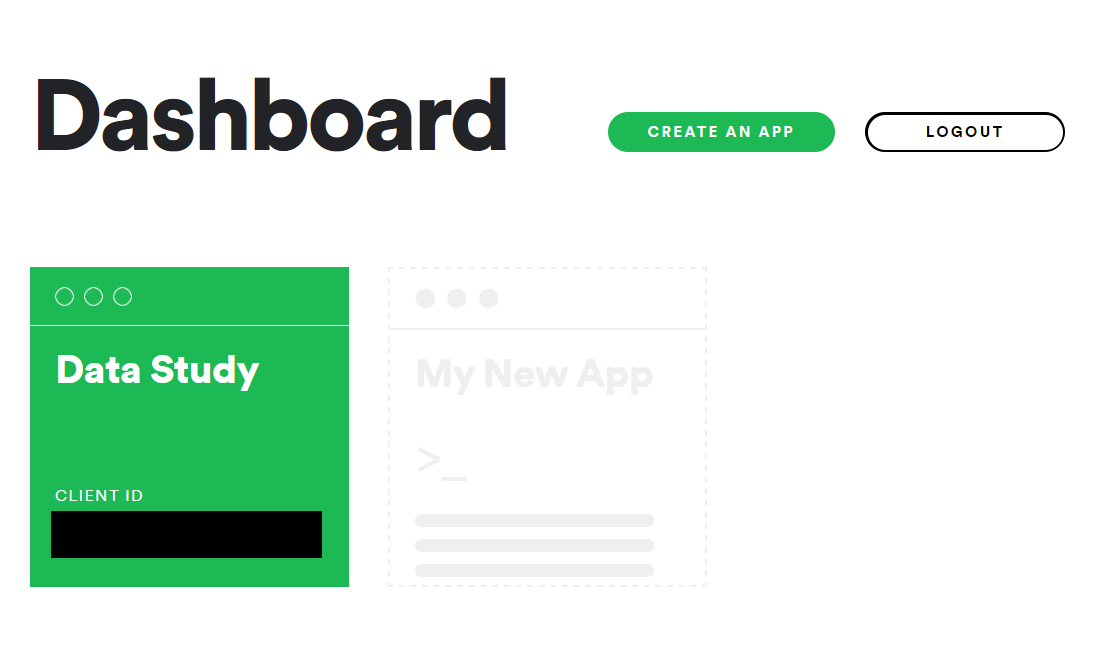
\includegraphics[width=120mm]{spotify_dev_dashboard.png}
    \caption{Spotify dashboard}
\end{figure}

\begin{figure}[h!]
    \centering
	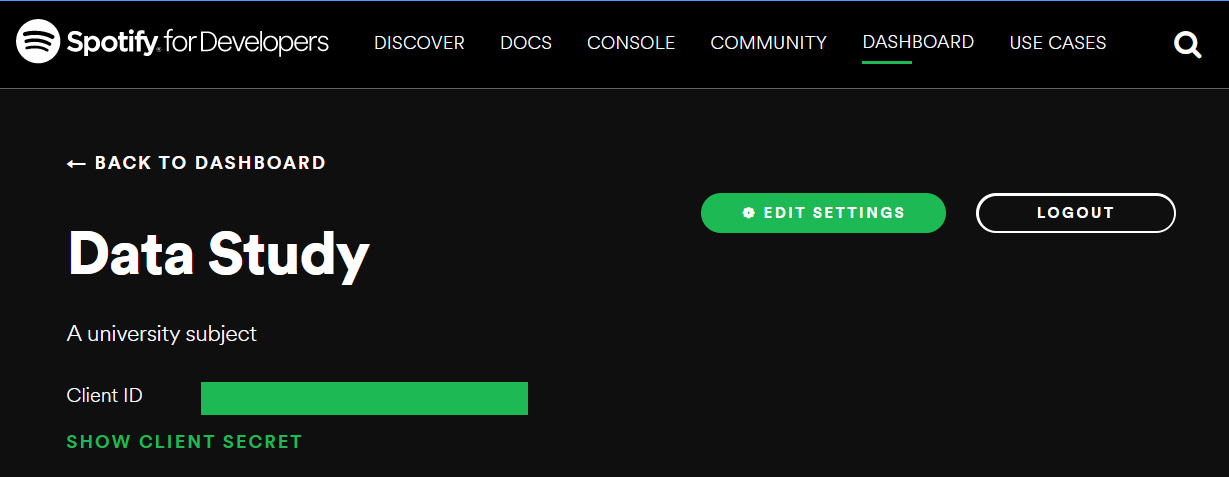
\includegraphics[width=120mm]{devoloper_spotify_1.png}
    \caption{Spotify application}
\end{figure}

\paragraph*{Una vez tengamos nuestra aplicacion creada necesitaremos el client ID y el client secret para poder autenticarnos 
y recuperar datos de la API.}

\paragraph*{Nuestro trabajo se compone de dos programas, el primero escrito en python utilizando Visual Studio Code
que nos permite recuperar datos de la API de Spotify y exportarlos a JSON. 
Y el segundo escrito en SageMath que nos permite representar y estudiar esos datos con teoría de grafos.}



\end{document}
